\ylDisplay{Optiline skeem} % Ülesande nimi
{Erkki Tempel} % Autor
{lahtine} % Voor
{2014} % Aasta
{G 7} % Ülesande nr.
{7} % Raskustase
{
% Teema: Geomeetriline-optika
\ifStatement
\begin{wrapfigure}{r}{0.5\textwidth}
 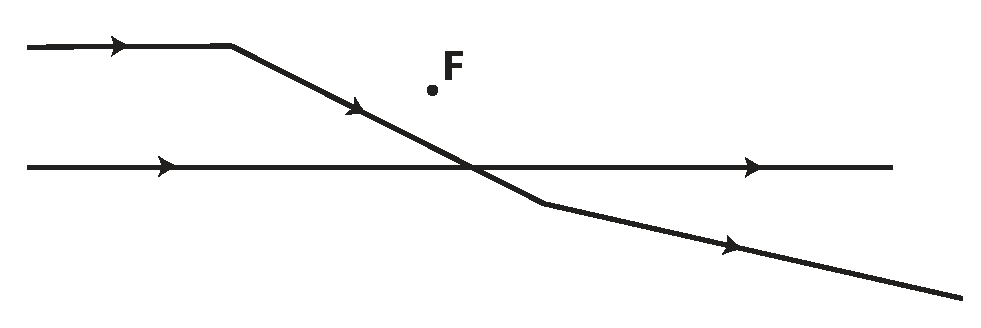
\includegraphics[width=0.5\textwidth]{2014-lahg-07-optilineskeemjoonis}
\end{wrapfigure}
Kõrvaloleval joonisel on kujutatud kahe algselt paralleelse kiire käik läbi kahe ühesuguse kumerläätse, mis ei asetse paralleelselt. Läätsede fookused ühtivad ning asuvad punktis F. Konstrueerige skeemile läätsed koos optiliste peatelgedega.
\fi


\ifHint
Algselt paralleelsed kiired koonduvad pärast läätse läbimist fokaaltasandis. Seega on võimalik esimese läätse fokaaltasand rekonstrueerida, teades fookuse asukohta ja kahe kiire lõikepunkti.
\fi


\ifSolution
\begin{center}
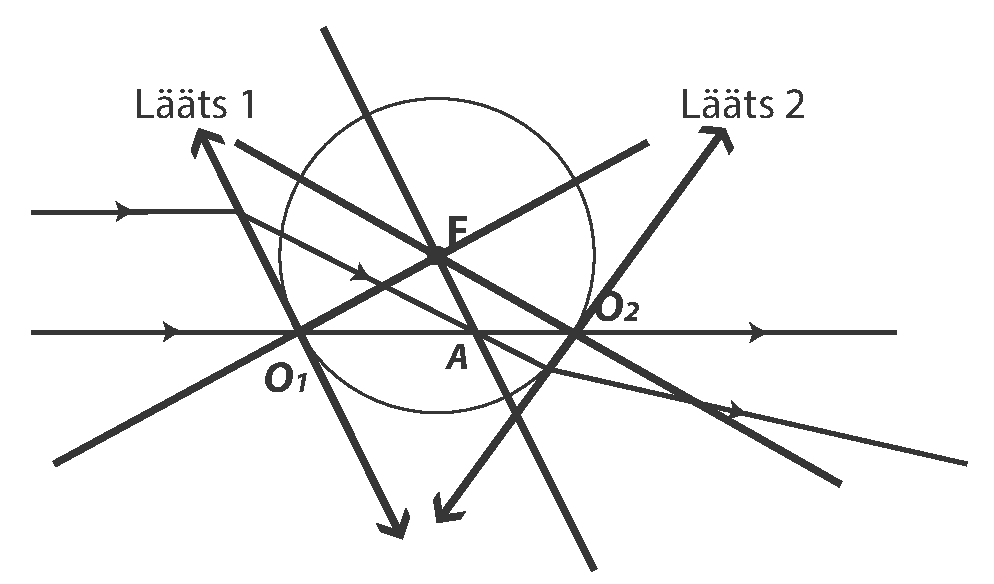
\includegraphics[width=0.7\textwidth]{2014-lahg-07-optilineskeemlahendus}
\end{center}
Algselt paralleelsed kiired koonduvad pärast läätse läbimist fokaaltasandis (punkt A). Kuna alumine kiir ei murdu, peab see läbima läätse keskpunkti. Seega lääts 1 on paralleelne joonistatud fokaaltasandiga (kiir läbib punkte A ja F) ning läbib punkti $\text{O}_1$. Kuna tegemist on kahe ühesuguse läätsega ning nende fookused asuvad punktis F, siis ring raadiusega $\text{FO}_1$ läbib alumist kiirt punktis $\text{O}_2$, mis on teise läätse keskpunktiks. Nüüd saame kergesti joonistada ka teise läätse, kuna teame ülemise kiire murdumiskohta ning läätse keskpunkti asukohta.
\fi


\ifEngStatement
% Problem name: Optical diagram
\begin{center}
  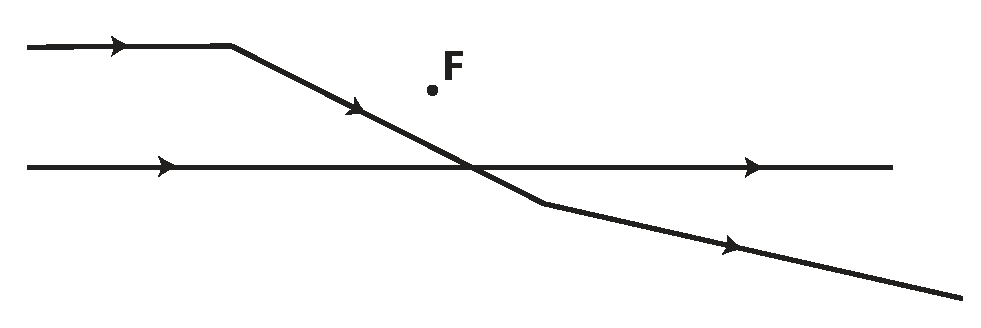
\includegraphics[width=0.7\textwidth]{2014-lahg-07-optilineskeemjoonis}
\end{center}
The figure depicts a route of two parallel beams through two identical convex lenses that are not parallel. The focal points of the lenses coincide at a point F. Construct the lenses with the optical axes on the figure.
\fi


\ifEngHint
Initially parallel rays focus on the focal plane after going through the lens. Thus it is possible reconstruct the focal plane of the first lens knowing the location of the focal point and the intersection point of two rays.
\fi


\ifEngSolution
\begin{center}
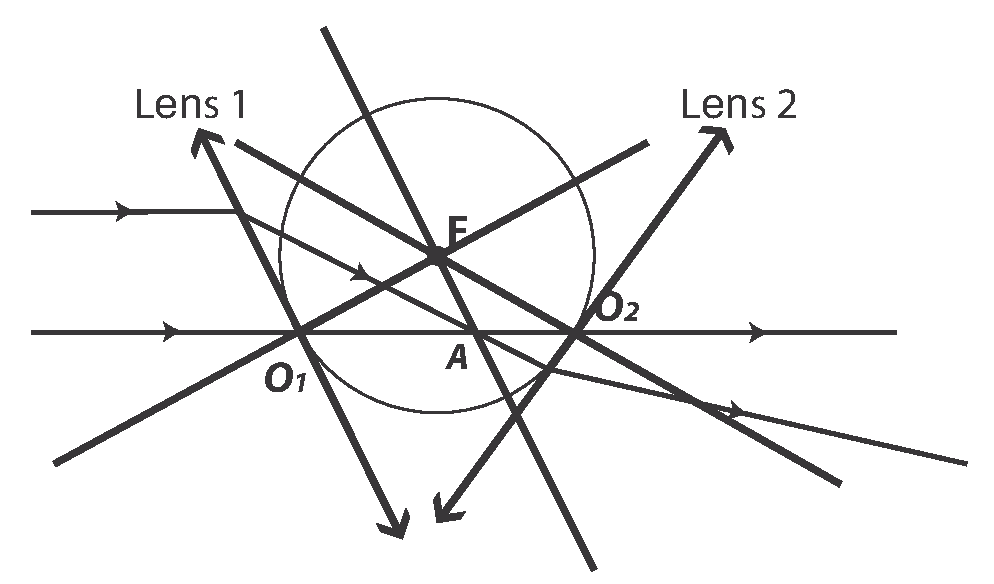
\includegraphics[width=0.7\textwidth]{2014-lahg-07-optilineskeemlahendus_ing}
\end{center}
Initially parallel rays converge on the focal plane (point A) after going through the lens. Because the bottom ray does not refract it has to go through the center of the lens. Therefore the lens 1 is parallel to the drawn focal plane (the ray goes through the points A and F) and goes through the point $\text{O}_1$. Because we are dealing with two identical lens and their focal points are at the point F then a circle of radius $\text{FO}_1$ intersects with the bottom ray at the point $\text{O}_2$ which is the center of the second lens. Now we can easily draw the second lens because we know the location of the bottom ray’s refraction point and the lens’ center.
\fi
}